% !LW recipe=LaTeXmk
\documentclass[11pt]{article}

\usepackage[margin=1in]{geometry}
\usepackage{amsmath}
\usepackage{booktabs}
\usepackage{graphicx}
\usepackage{microtype}
\usepackage[compact]{titlesec}
\usepackage[hidelinks]{hyperref}
\setlength{\textfloatsep}{8pt plus 2pt}
\setlength{\intextsep}{8pt plus 2pt}
\setlength{\abovecaptionskip}{4pt}

\title{SnapReady: A Webcam Coach for Passport Photos\\[0.2em] \large CIS 5810 Final Project Midterm Report (Option 1)}
\author{\normalsize Group 37\\[0.2em]
\normalsize
\begin{tabular}{ccc}
Susan Xiong & Kai Wang & Yincheng Zhou \\
\small\texttt{xiongs@sas.upenn.edu} & \small\texttt{kai6@sas.upenn.edu} & \small\texttt{yzhou29@engineering.upenn.edu}
\end{tabular}}
\date{}

\begin{document}
\maketitle
\vspace{-2.5em}

\paragraph{Summary} SnapReady helps a person take a valid US passport photo with a webcam. It measures the face in every frame, tells the user the one thing to fix, takes the photo by itself once every rule passes, and returns a $600 \times 600$ photo on white. Since the proposal we made three changes. The app now runs as a live browser interface. The benchmark now uses aligned photos with clean labels, so its numbers can be trusted. The model now measures each rule on the part of the face it is about. On the new benchmark SnapReady beats the baseline on all seven checks.

\section{Pipeline design}

Every frame goes through MediaPipe's Face Landmarker~\cite{mediapipe}, which gives 478 face landmarks, blink scores and head pose. \textbf{Check} turns these into 11 measurements: distance from the iris size (pinhole model), face size and position, head turn, nod and tilt, eye closure, brightness, side shadow and sharpness. \textbf{Guide} compares each measurement to a limit and shows the first failing rule in a fixed order, so big moves come before small ones. When every rule passes for 20 frames in a row it keeps the sharpest frame. \textbf{Finish} levels the eyes and scales the head with a similarity transform, cuts the person out with the Selfie Segmenter, and blends the person onto white with a Laplacian pyramid. All limits except distance and face size are fitted by grid search on a calibration half of the data and scored on the other half by balanced accuracy, the mean of bad photos caught and good photos passed.

\section{Baseline results}
\label{sec:baseline}

Our baseline uses Viola-Jones Haar cascades~\cite{viola2001} for the face and eyes, with whole-image brightness and sharpness. It cannot measure head turn or nod. It goes through the same limit fitting, so the only difference is the measurements.

\begin{table}[h]
\centering
\footnotesize
\begin{tabular}{@{}lccccccc@{}}
\toprule
 & Centered & Sharp & Exposure & Even light & Head level & Facing & Eyes open \\
\midrule
\multicolumn{8}{@{}l}{\emph{Proposal: prototype benchmark}} \\
Baseline (Viola-Jones) & \textbf{99.4} & \textbf{90.2} & 88.6 & 78.2 & 74.0 & 78.8 & 77.0 \\
SnapReady              & 96.2 & 87.4 & \textbf{94.9} & \textbf{81.1} & \textbf{79.7} & \textbf{90.5} & \textbf{100.0} \\
\midrule
\multicolumn{8}{@{}l}{\emph{Midterm: new benchmark}} \\
Baseline (Viola-Jones) & 97.4 & 91.5 & 87.1 & 92.0 & 75.8 & 78.8 & 79.9 \\
SnapReady              & \textbf{98.2} & \textbf{92.4} & \textbf{97.0} & \textbf{94.8} & \textbf{89.5} & \textbf{90.5} & \textbf{97.2} \\
\bottomrule
\end{tabular}
\caption{Balanced accuracy (\%) on the test half of each benchmark. 50\% is guessing. The two benchmarks use different data, so the rows are not directly comparable across stages.}
\label{tab:results}
\end{table}

On the new benchmark the baseline is strong where a face box is enough: centering, sharpness and even light. It is weak where it needs the shape of the face. With head turn and nod fixed at zero, it only catches a turned head when it loses the face altogether, and it finds the eyes only as boxes, so tilt and closed eyes are hard for it. Exposure suffers because it averages the whole image instead of the face.

\section{Development iterations and results}

We ran three iterations on top of the proposal version. Each one was tested before the next one started.

\subsection{Iteration 1: a live interface}

SnapReady now runs in the browser with Gradio~\cite{gradio}, so anyone can open a link and use it (Fig.~\ref{fig:interface}). The live tab shows the camera, the same view with the face outline and the current instruction, and a bar that fills while the user holds still. Under it a table lists all 11 rules with the measured value, the allowed range and a pass or fail mark, so it is clear why a rule fails. The finished photo appears when it is taken. A second tab checks and finishes an uploaded photo. We flip the browser's mirrored frames back before measuring, so left and right instructions are not reversed. \textbf{Result.} When we stream test photos through the live tab frame by frame, the instruction follows the face and the photo is taken after exactly 20 passing frames.

\begin{figure}[h]
\centering
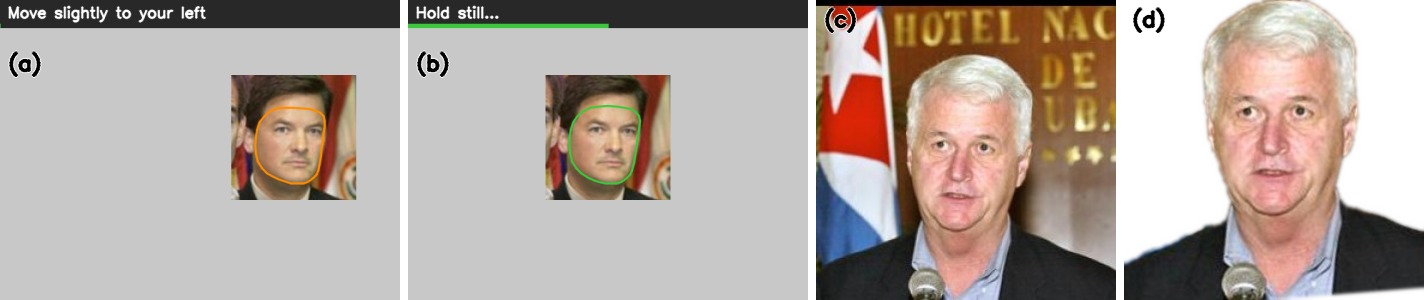
\includegraphics[width=0.88\linewidth]{figures/interface.jpg}
\caption{(a) The live tab tells the user to move. (b) All rules pass and the bar fills before the photo is taken. Both use a test photo in a webcam-sized frame. (c, d) The photo tab turns an LFW photo into a passport photo.}
\label{fig:interface}
\end{figure}

\subsection{Iteration 2: a benchmark we can trust}
\label{sec:benchmark}

The prototype test damaged LFW~\cite{lfw} photos on purpose and assumed every undamaged photo was a good passport photo, which was often wrong. With our final measurements, 19\% of the undamaged photos were tilted past the limit and 20\% were lit from one side, so both models were often penalized for being right. The raw photos had also been cropped around a Haar face box, which favors the baseline on framing, and they were enlarged from 180 to 320 pixels, which blurred every ``sharp'' photo before any blur was added. The eyes test also used only AI-generated faces~\cite{eyesdata}. The eye limit fitted there marked 44\% of real people with open eyes as closed, mostly people who squint when they smile.

We fixed the data rather than the model. We switched to funneled LFW, where every face was aligned by congealing~\cite{funnel}, a method that uses neither our landmarks nor Haar. We keep the photos at their own size. We even out the lighting of each photo before adding damage: we treat the image as detail times light, take the light to be a heavy blur, and replace it by the geometric mean of itself and its mirror image. The face looks the same, but the side light is gone. We also added the undamaged LFW photos to the eyes test as real open eyes. Facing is still tested on Pointing'04 head poses~\cite{pointing04}. \textbf{Result.} The share of good photos tilted past the limit fell from 19\% to 5.8\%, and the share lit from one side fell from 20\% to 4.5\%, so the remaining errors mostly belong to the models. The new benchmark then showed clearly where our own model was weak.

\subsection{Iteration 3: a stronger model}

Each rule now looks at the part of the face it is about, and where it can, compares two things that should be equal (Fig.~\ref{fig:measure}).

\begin{itemize}
    \setlength{\itemsep}{0pt}
    \item \textbf{Position} is the midpoint of the outer eye corners relative to the image center. The passport rule places the eye line, and the eye corners are the steadiest landmarks, while the face outline shifts with the jaw and head turn.
    \item \textbf{Brightness} is the 90th percentile of the face pixels. Exposure shows in the lit skin, while a median would be pulled down by beards, eyebrows and shadows.
    \item \textbf{Side shadow} compares the mean brightness in small patches around nine mirrored cheek landmarks, found with a box filter, as the ratio of the brighter side to the darker side. Under even light the same skin on both cheeks is equally bright, so comparing like with like keeps hair, background and head turn out of the measurement.
    \item \textbf{Sharpness} blurs the face once more with a Gaussian and measures the share of edge strength (Sobel gradient magnitude) that the blur removes~\cite{crete2007}. A sharp face has fine edges that the blur wipes out, while a blurry face has little left to lose. Since it is a ratio, a darker or flatter face gives the same value, and we resize the face to a fixed width so the distance to the camera does not matter either.
    \item \textbf{Tilt} is the mean angle of five lines joining mirrored landmarks: the outer and inner eye corners, the mouth corners, the sides of the face and the brows. Each line alone carries a little landmark noise, and the average is steadier.
    \item \textbf{Eyes open} uses the larger of MediaPipe's two blink scores, with the limit fitted on real faces as well as AI faces.
    \item \textbf{Finish} keeps only the part of the person mask that is connected to the face, so people standing behind the user are removed.
\end{itemize}

\begin{figure}[h]
\centering
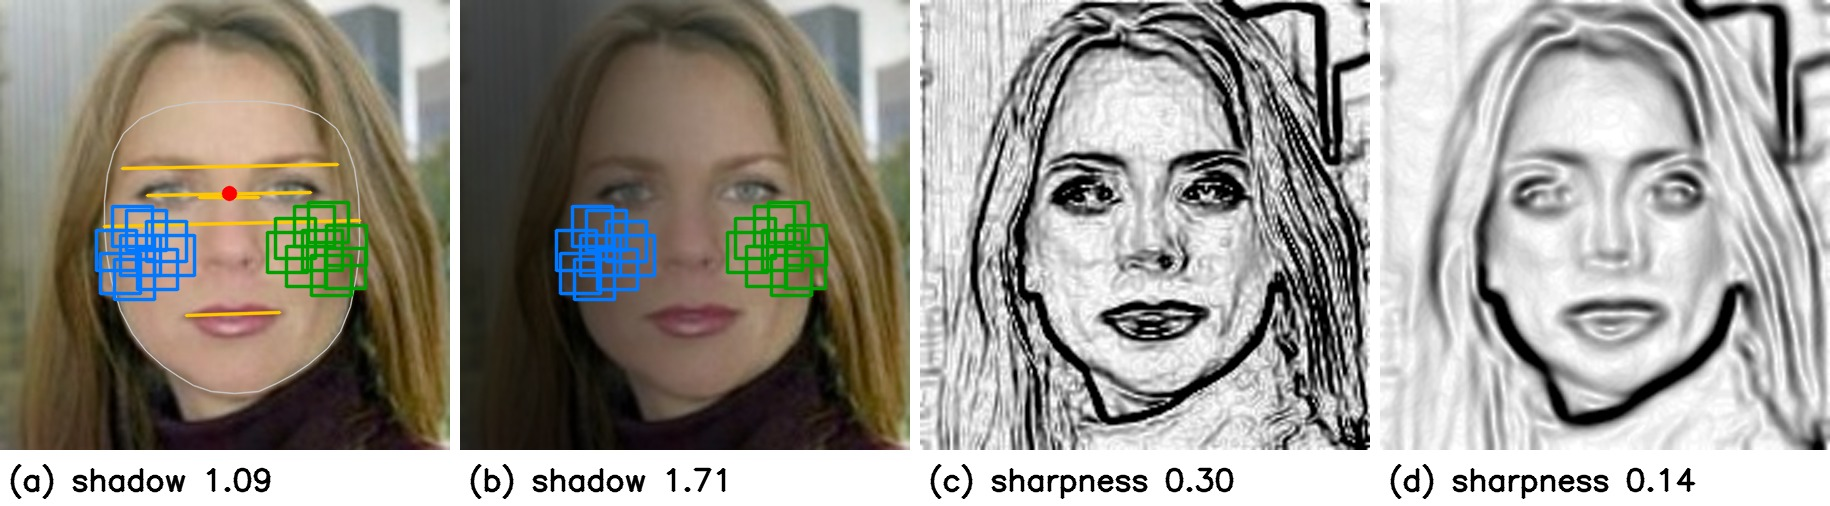
\includegraphics[width=0.85\linewidth]{figures/measurements.jpg}
\caption{What the model measures. (a) The yellow lines give the tilt, the red dot the position, and the boxes are the cheek patches for side shadow. (b) A side shadow pushes the ratio over its limit of 1.35. (c, d) Edge strength when sharp and when blurred. Sharpness, the share of edge strength that one more blur removes, falls below its limit of 0.21 in (d).}
\label{fig:measure}
\end{figure}

\textbf{Result.} At the proposal SnapReady won five of seven checks and lost centering and sharpness, the two checks that the prototype data biased (Section~\ref{sec:benchmark}). It now beats the baseline on all seven (Table~\ref{tab:results}), and the largest gains are on the four checks where Section~\ref{sec:baseline} found the baseline weak: tilt, facing, eyes and exposure.

\paragraph{What is still weak} A person who touches the user stays in the photo, and dark backgrounds leave a dark edge around the hair.

\section{Goals, audience and plan}

Our audience is anyone who needs a passport or visa photo and would rather take it at home. The goal is a photo that passes the official rules on the first try, without the user having to learn them.

\paragraph{Timeline, milestones and duties} By 11/30 we will record our own webcam test set with scripted mistakes, check the limits on it, and fix the hair edge in Finish. By 12/6 we will run a small user study that times how long it takes to get a valid photo with SnapReady and with a normal camera app, and prepare the demo.
Yincheng Zhou: Check, benchmark and limit fitting. Susan Xiong: Guide, the live interface and the user study. Kai Wang: Finish and the webcam test set.

\paragraph{Credits and AI use} MediaPipe Face Landmarker and Selfie Segmenter (Apache 2.0), OpenCV Haar cascades, Gradio. Code: \url{https://github.com/ArtysicistZ/SnapReady}; \texttt{benchmark.py} reproduces Table~\ref{tab:results}. We used Claude Code (Anthropic) to assist brainstorming, debug the code, and draft this report.

{\footnotesize
\begin{thebibliography}{9}
\setlength{\itemsep}{0pt}
\bibitem{viola2001} P. Viola, M. Jones. Rapid object detection using a boosted cascade of simple features. CVPR 2001.
\bibitem{mediapipe} Y. Kartynnik et al. Real-time facial surface geometry from monocular video on mobile GPUs. CVPRW 2019.
\bibitem{gradio} A. Abid et al. Gradio: hassle-free sharing and testing of ML models in the wild. arXiv:1906.02569, 2019.
\bibitem{lfw} G. Huang et al. Labeled Faces in the Wild. UMass Tech. Report 07-49, 2007.
\bibitem{pointing04} N. Gourier et al. Estimating face orientation from robust detection of salient facial features. ICPRW 2004.
\bibitem{eyesdata} M. Mlodawski. closed-open-eyes. huggingface.co/datasets/MichalMlodawski/closed-open-eyes.
\bibitem{funnel} G. Huang, V. Jain, E. Learned-Miller. Unsupervised joint alignment of complex images. ICCV 2007.
\bibitem{crete2007} F. Cr\'ete-Roffet et al. The blur effect: a new no-reference perceptual blur metric. SPIE 2007.
\end{thebibliography}}

\end{document}
